%!TEX root = ../../../main.tex
%%---------------------------------------------------------------------------
\section{SCRUM \label{sec:scrum}}
%%---------------------------------------------------------------------------

%Description of our way of doing SCRUM...

The Agile methodology suited this project since the iterative development has a good synergy when it comes to customer collaboration and changes in requirements. Two aspects in the system development was influencing the breakdown of tasks to be completed before the system could be called finished. the first aspect was that the system requirements was not all defined from the beginning and the defined requirement could change over time. The second aspect was that allot of new technologies and tools which the team was unfamiliar with made it hard to get a breakdown of the processes required to complete the system.

The project started the 7th of September 2015 with a introduction to the system requirements by the product owners and the system development ended the 7th of December with a 24 hour integration test.

The team gathered after the system requirements was presented in order to create an initial prioritized product backlog. The team utilized Trello\footnote{https://trello.com/} in order to keep track of the tasks in the backlog. Trello is an online project management application and was used since its design made it similar to post-it notes for management and it also had the advantage of being online and was therefore accessible from both home and workplace through smart phones or computers. Figure \ref{fig:trello_cap} shows a screen capture of Trello opened in a browser.
\begin{figure}[H]
	\centering
	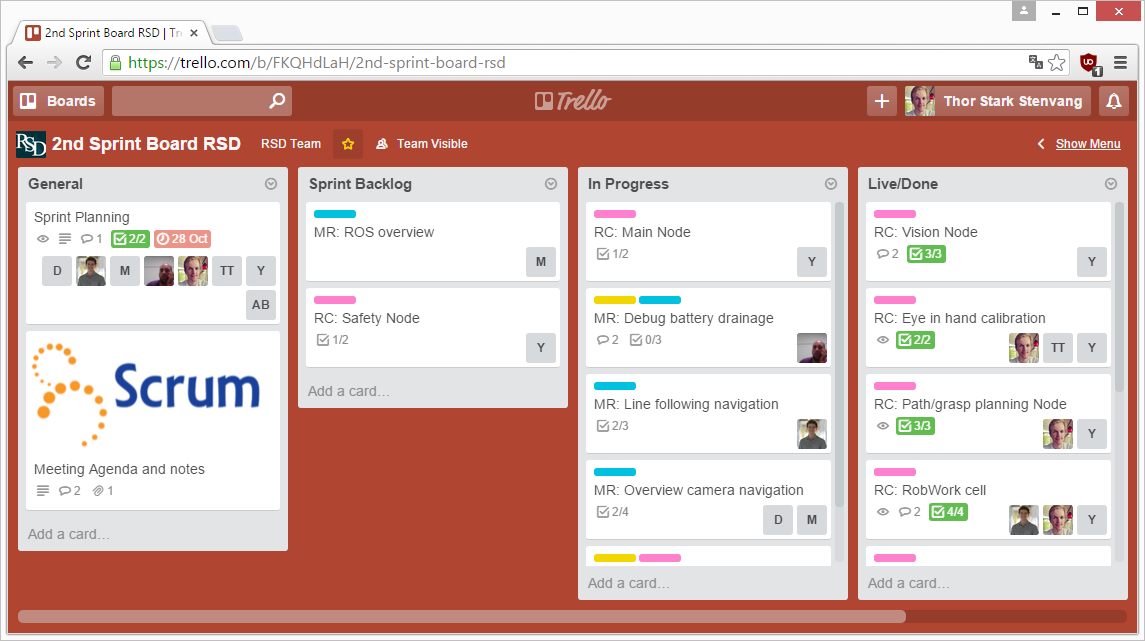
\includegraphics[width=\textwidth]{figs/trello_example.png}
	\caption{Screen capture of a Trello showing the Trello board for the 2nd Sprint. The three rightmost lists are used to keep track of tasks and their state.}
	\label{fig:trello_cap}
\end{figure}


\subsection{Sprints} \label{sec:sprints}
Over the course of the project the work was divided into 4 sprints. Each sprint planning except for the first was done after the completion of the previous. For each sprint planning a sprint goal and the duration of the sprint was decided. Prioritized tasks was then added to the Sprint backlog. When the Sprint was running each member could then sign up for a task and they will be distinguished between being completed or still in progress.
Listed below are the different Sprints and their description.
\begin{itemize}
    \item \textbf{1st Sprint.}
    \begin{itemize}
    	\item \textbf{Goal:} Create a working robot demo for the TEK opening and prepare the simple elements for the robot cell.
    	\item \textbf{Duration:} 14th of Sep - 30th of Sep.
    	\item \textbf{Description:} Additional to the system described in the original system requirements a additional system was suddenly to be developed with a release date of 30th of September. The Sprint was designed with the new requirements and deadline in mind. There was also several technologies not available at the moment of the sprint which made the amount of work could be done with the robot cell depending on when the technologies was ready. Allot of focus an work was therefore focused on the mobile robot.
	\end{itemize}
	
    \item \textbf{2nd Sprint.}
    \begin{itemize}
    	\item \textbf{Goal:} Fulfill the requirements for the hallfway demonstration.
    	\item \textbf{Duration:} 5th of Oct - 28th of Oct.
    	\item \textbf{Description:} Compared with the focused workload on the mobile robot in the previous sprint. This Sprint was spreading more of the workforce onto a broader part of the whole system. The reason for this was the requirements of the system for the halfway demonstration for the product owner. It was therefore with new tolls and technology possible to work on the robot work cell in addition to the mobile robot.
	\end{itemize}
	
    \item \textbf{3rd Sprint.}
    \begin{itemize}
    	\item \textbf{Goal:} Get the system ready so all subsystems and components can be integrated together in the next sprint.
    	\item \textbf{Duration:} 28th of Oct - 18th of Nov.
    	\item \textbf{Description:} With most of the work on the robot work cell done in the previous sprint. The workforce was shifted so more people was working on the mobile robot in order for it to be ready for implementation and integration in the whole system.
	\end{itemize}
	
    \item \textbf{4th Sprint.}
    \begin{itemize}
    	\item \textbf{Goal:} Integrate all subsystems and components and prepare for the 24 hour integration test.
    	\item \textbf{Duration:} 23rd of Nov - 7th of Dec.
    	\item \textbf{Description:} Line following, relative navigation, free navigation etc.. was integrated together so they in conjugation can perform all the defined task for the mobile robot. Bug fixes and recovery behaviour was also done in order to complete the 24 hour integration test in an environment where other robots are present.
	\end{itemize}
\end{itemize}

In order to keep an overview of the project and keeping it on track a weekly SCRUM meeting was held together with the Consultant and a Product owner. Summery of the meetings can maybe be found in appendix ??, it depends on if we have added them there.




%Following is a list of addition and changes in system requirements:
%\begin{itemize}
%    \item Addition: A version of the mobile robot being able to cross a specified bridge should be developed and be ready for deployment at the TEK opening the 30th of September 2015.
%    \item ???
%\end{itemize}